
\newpage
\thispagestyle{fancy}
\vspace*{40 pt}
\subsection{Tela de comandos Empilhador} \label{sec:telaComandosEmpilhador}
Esta tela é acessada pelo botão direito "\textgreater" na tela de comando empilhador.
\vspace*{\fill}
\begin{figure}[h]
    \centering
    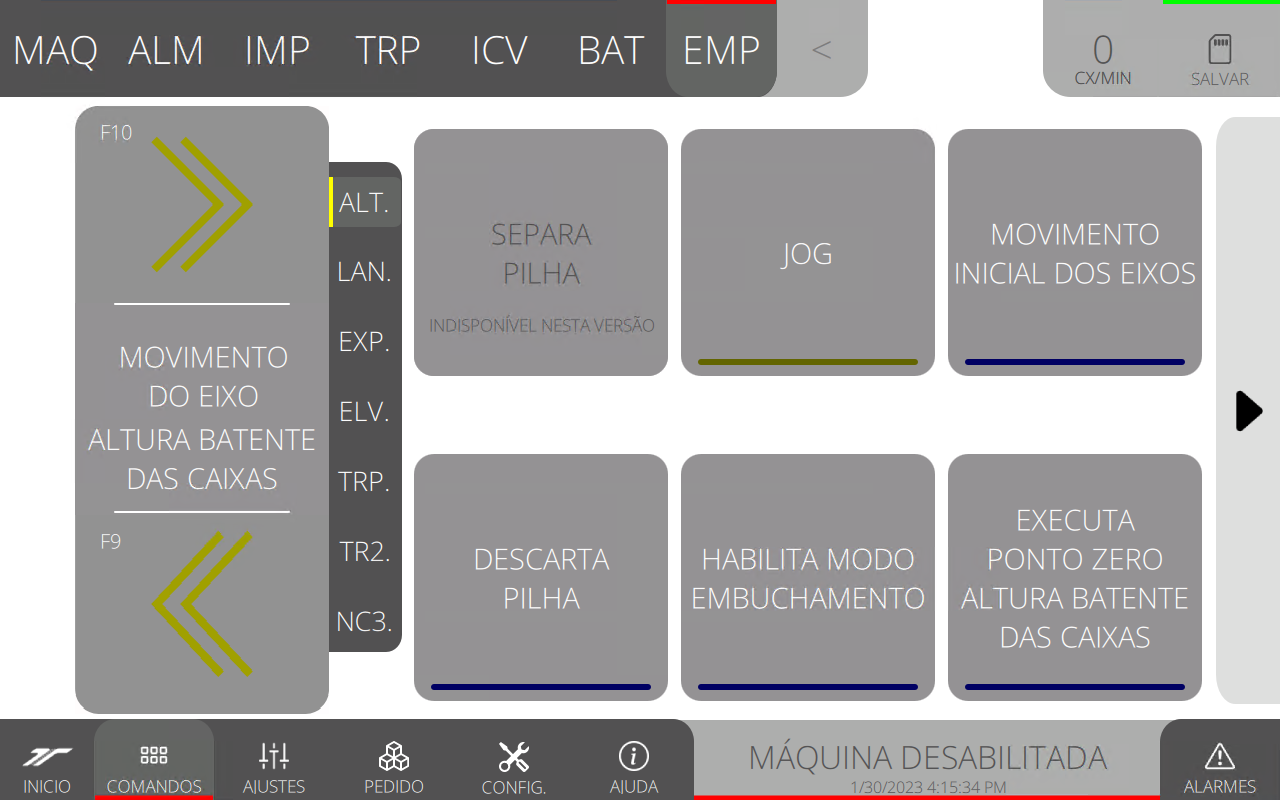
\includegraphics[width=480 px,height=300 px]{src/imagesICV/08-stacker/commands/Tela-Principal.png}
\end{figure}
\vspace*{\fill}

\newpage
\thispagestyle{fancy}
\vspace*{40 pt}
\subsubsection{\small{Movimento dos eixos}} \label{sec:telaComandosEmpilhadorMovimentoEixos}
\vspace*{\fill}
\begin{figure}[h]
    \centering
    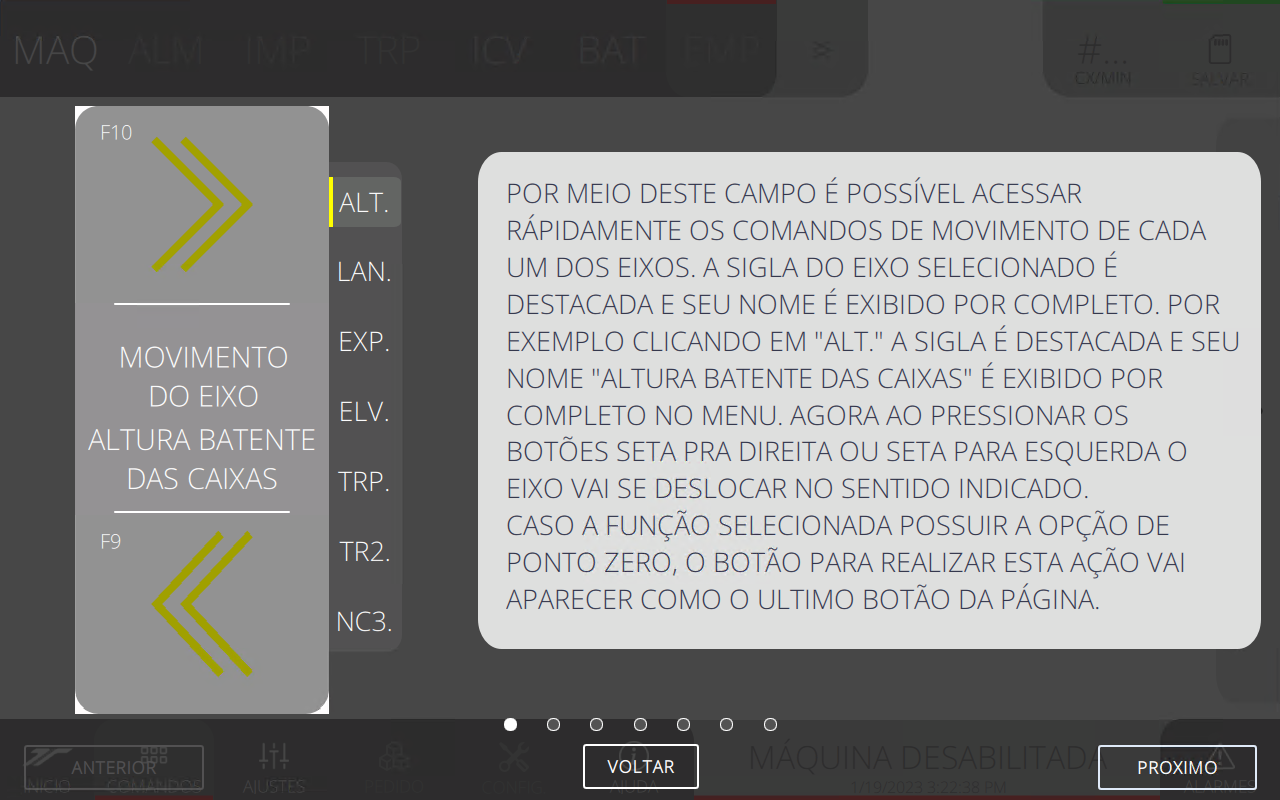
\includegraphics[width=576 px,height=360 px]{src/imagesICV/08-stacker/commands/e-6.png}
\end{figure}
\vspace*{\fill}

\newpage
\thispagestyle{fancy}
\vspace*{40 pt}
\subsubsection{\small{Executa ponto zero altura batente das caixas}} \label{sec:telaComandosEmpilhadorExecutaPontoZeroAlturaBatenteCaixas}
\vspace*{\fill}
\begin{figure}[h]
    \centering
    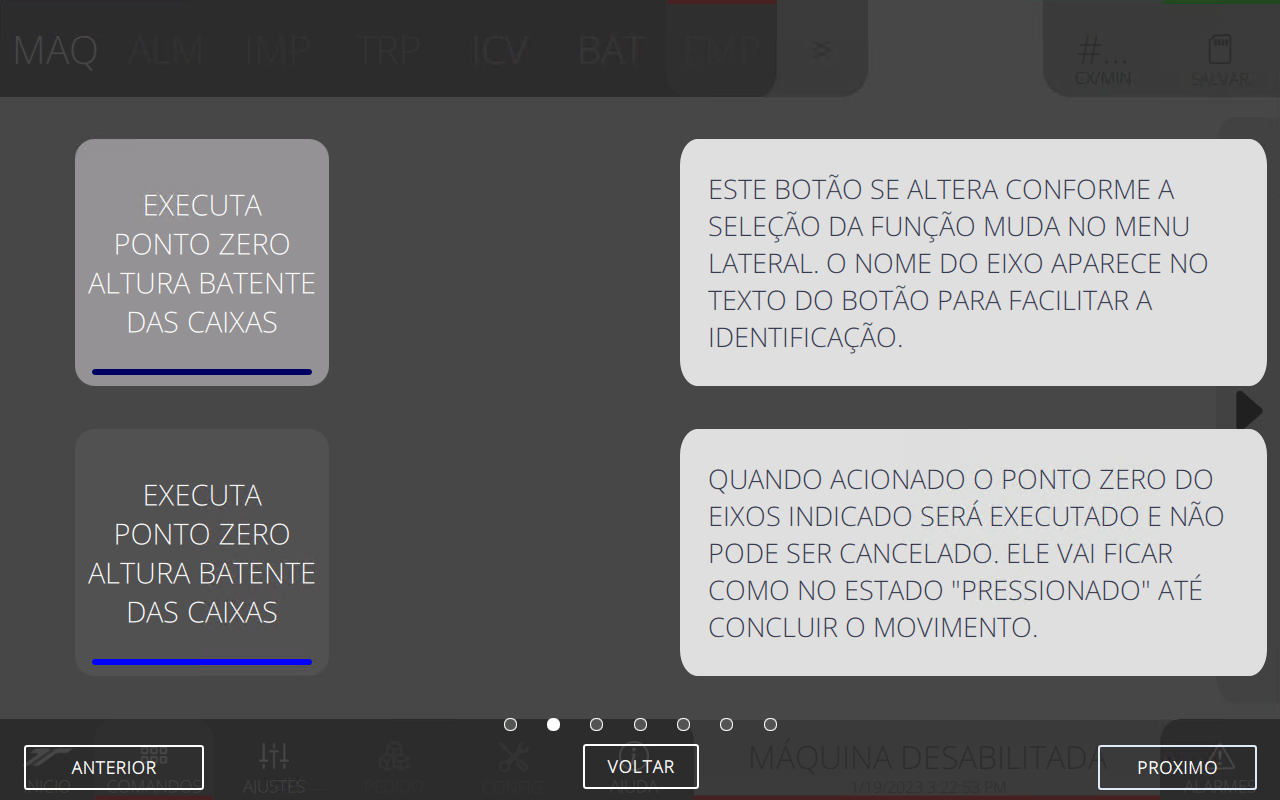
\includegraphics[width=576 px,height=360 px]{src/imagesICV/08-stacker/commands/e-7.png}
\end{figure}
\vspace*{\fill}

\newpage
\thispagestyle{fancy}
\vspace*{40 pt}
\subsubsection{\small{Habilita função Jog}} \label{sec:telaComandosEmpilhadorHabilitaFuncaoJog}
\vspace*{\fill}
\begin{figure}[h]
    \centering
    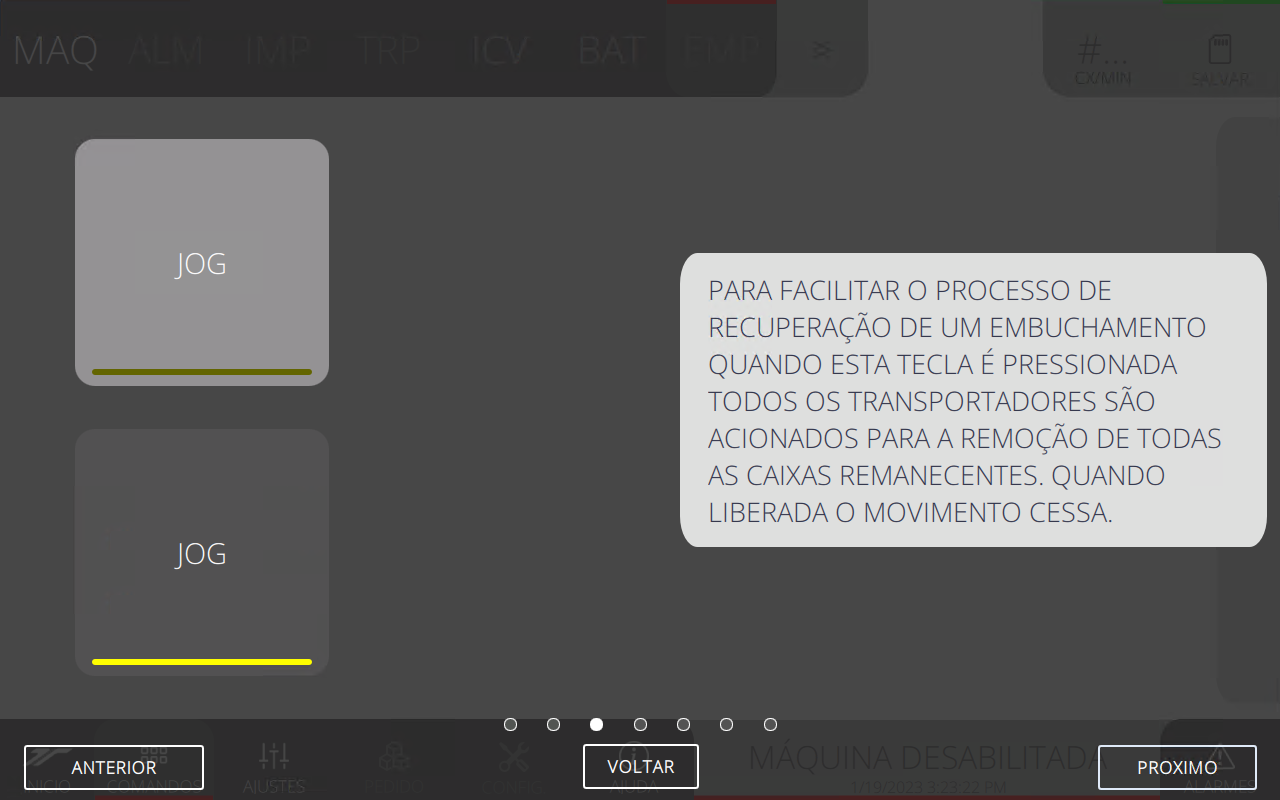
\includegraphics[width=576 px,height=360 px]{src/imagesICV/08-stacker/commands/e-8.png}
\end{figure}
\vspace*{\fill}

\newpage
\thispagestyle{fancy}
\vspace*{40 pt}
\subsubsection{\small{Movimento incial dos eixos}} \label{sec:telaComandosEmpilhadorMovimentoInicialEixos}
\vspace*{\fill}
\begin{figure}[h]
    \centering
    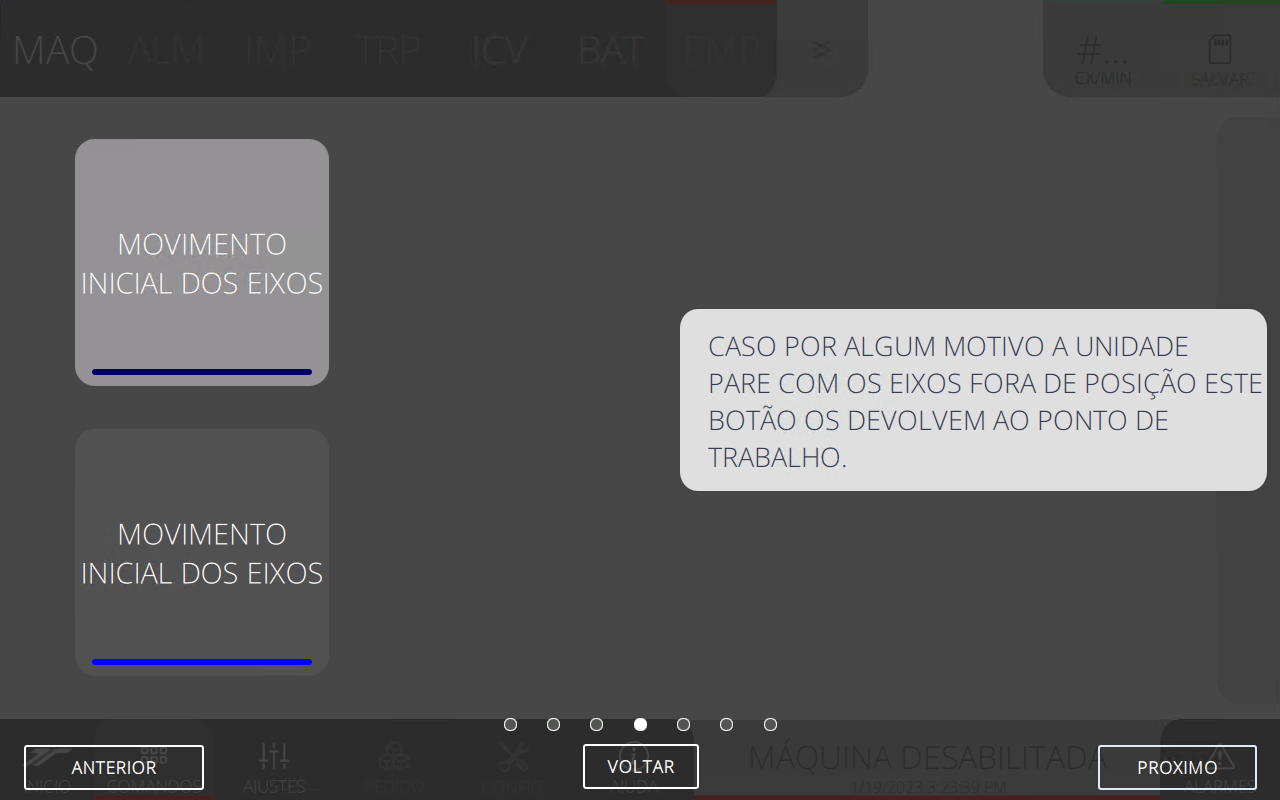
\includegraphics[width=576 px,height=360 px]{src/imagesICV/08-stacker/commands/e-9.png}
\end{figure}
\vspace*{\fill}

\newpage
\thispagestyle{fancy}
\vspace*{40 pt}
\subsubsection{\small{Descarta pilha}} \label{sec:telaComandosEmpilhadorDescartaPilha}
\vspace*{\fill}
\begin{figure}[h]
    \centering
    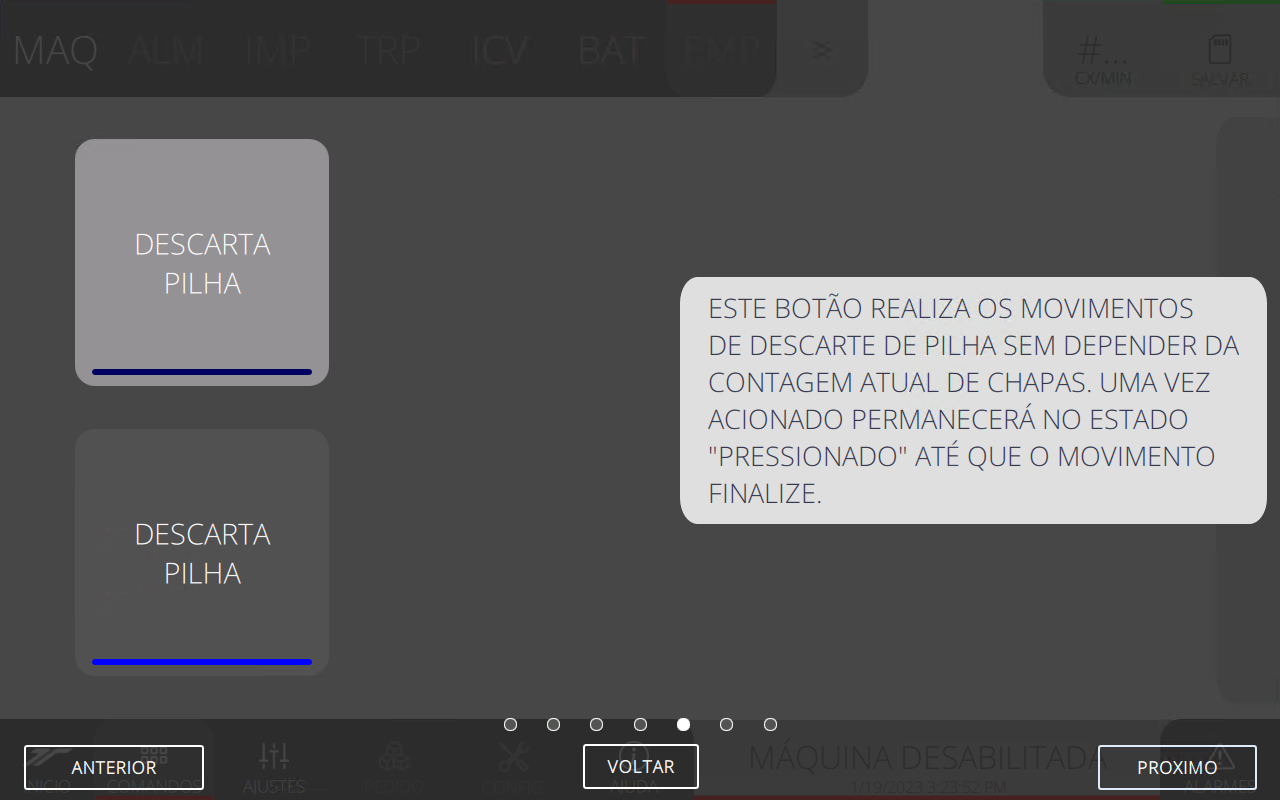
\includegraphics[width=576 px,height=360 px]{src/imagesICV/08-stacker/commands/e-10.png}
\end{figure}
\vspace*{\fill}

\newpage
\thispagestyle{fancy}
\vspace*{40 pt}
\subsubsection{\small{Habilita modo embuchamento}} \label{sec:telaComandosEmpilhadorHabilitaModoEmbuchamento}
\vspace*{\fill}
\begin{figure}[h]
    \centering
    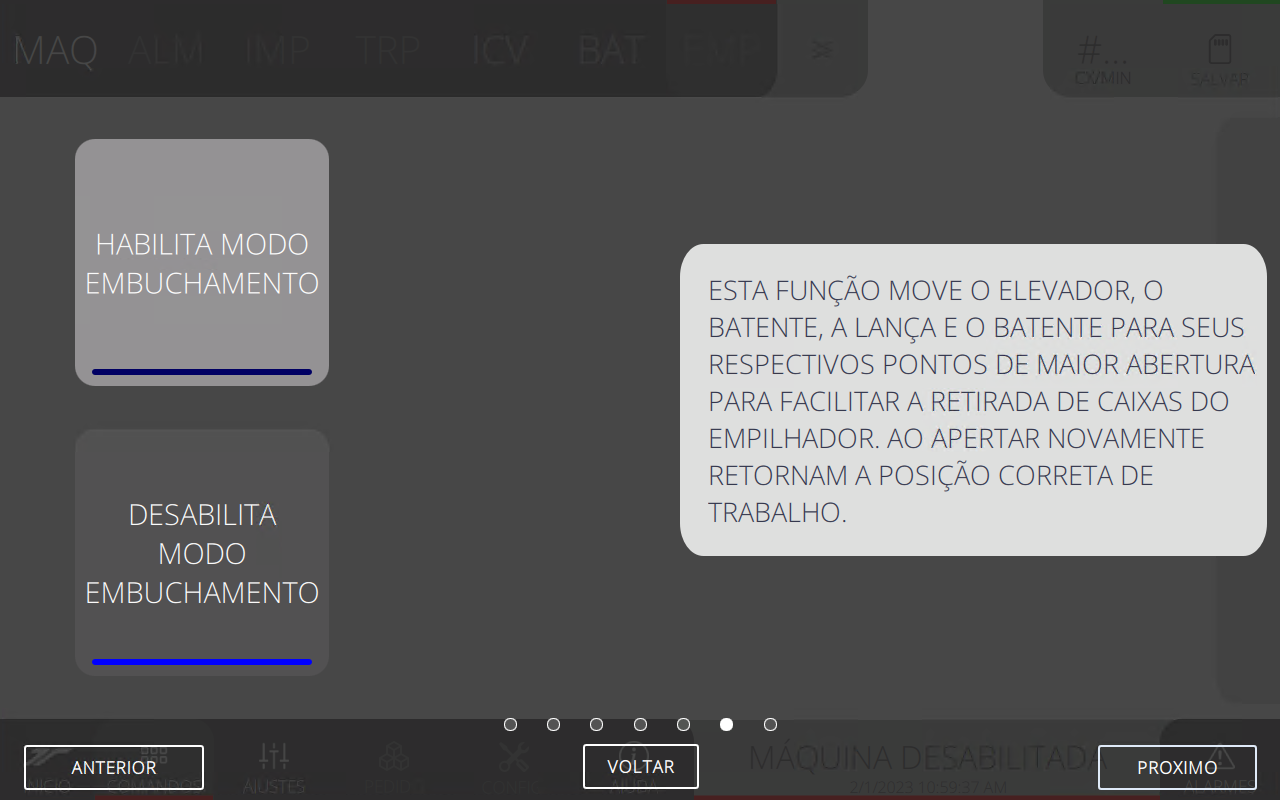
\includegraphics[width=576 px,height=360 px]{src/imagesICV/08-stacker/commands/e-11.png}
\end{figure}
\vspace*{\fill}

\newpage
\thispagestyle{fancy}
\vspace*{40 pt}
\subsubsection{\small{Separa pilha}} \label{sec:telaComandosEmpilhadorSeparaPilha}
\vspace*{\fill}
\begin{figure}[h]
    \centering
    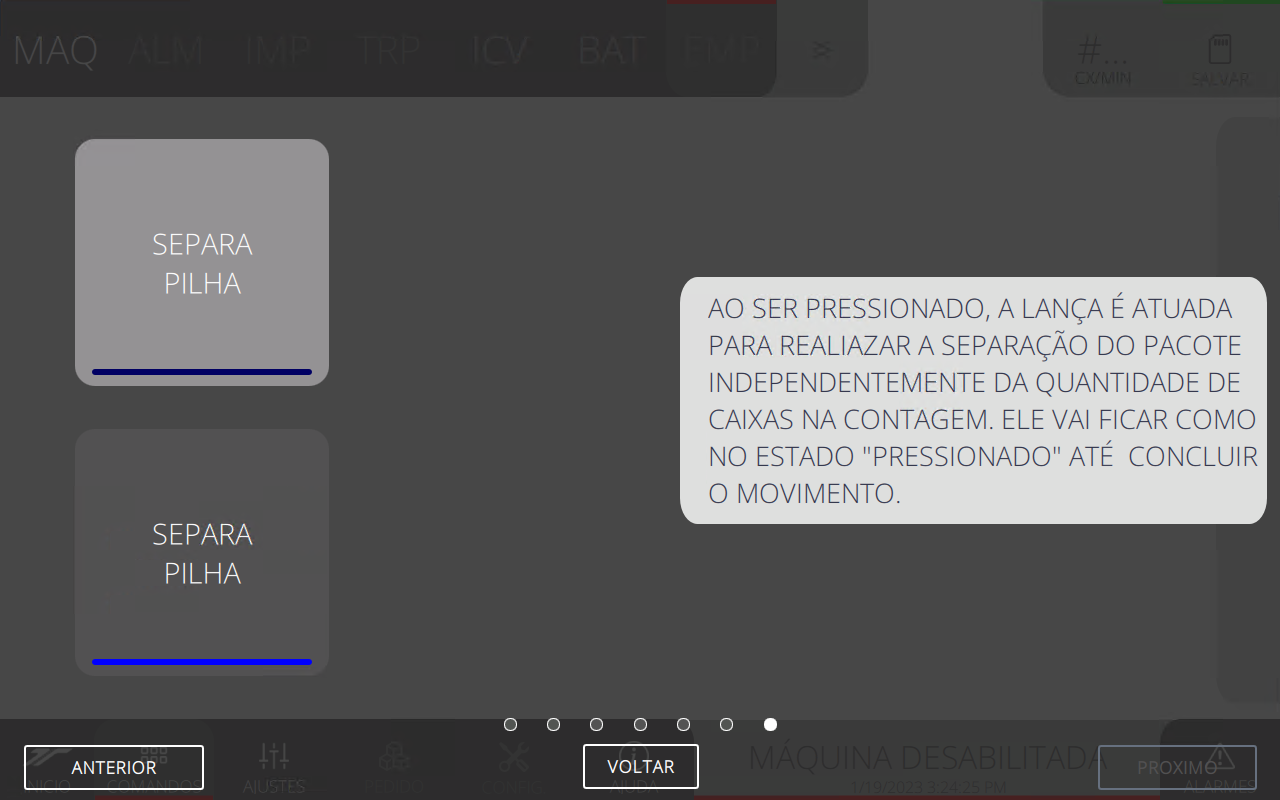
\includegraphics[width=576 px,height=360 px]{src/imagesICV/08-stacker/commands/e-12.png}
\end{figure}
\vspace*{\fill}

\newpage
\thispagestyle{fancy}
\vspace*{40 pt}
\subsection{Segunda tela de comandos Empilhador} \label{sec:telaComandosEmpilhador2}
Esta tela é acessada pelo botão "\textgreater" no menu superior esquerdo da tela de comando batedor, pelo botão "EMP" em qualquer tela de comando e pelo botão comando da tela ajustes empilhador.
\vspace*{\fill}
\begin{figure}[h]
    \centering
    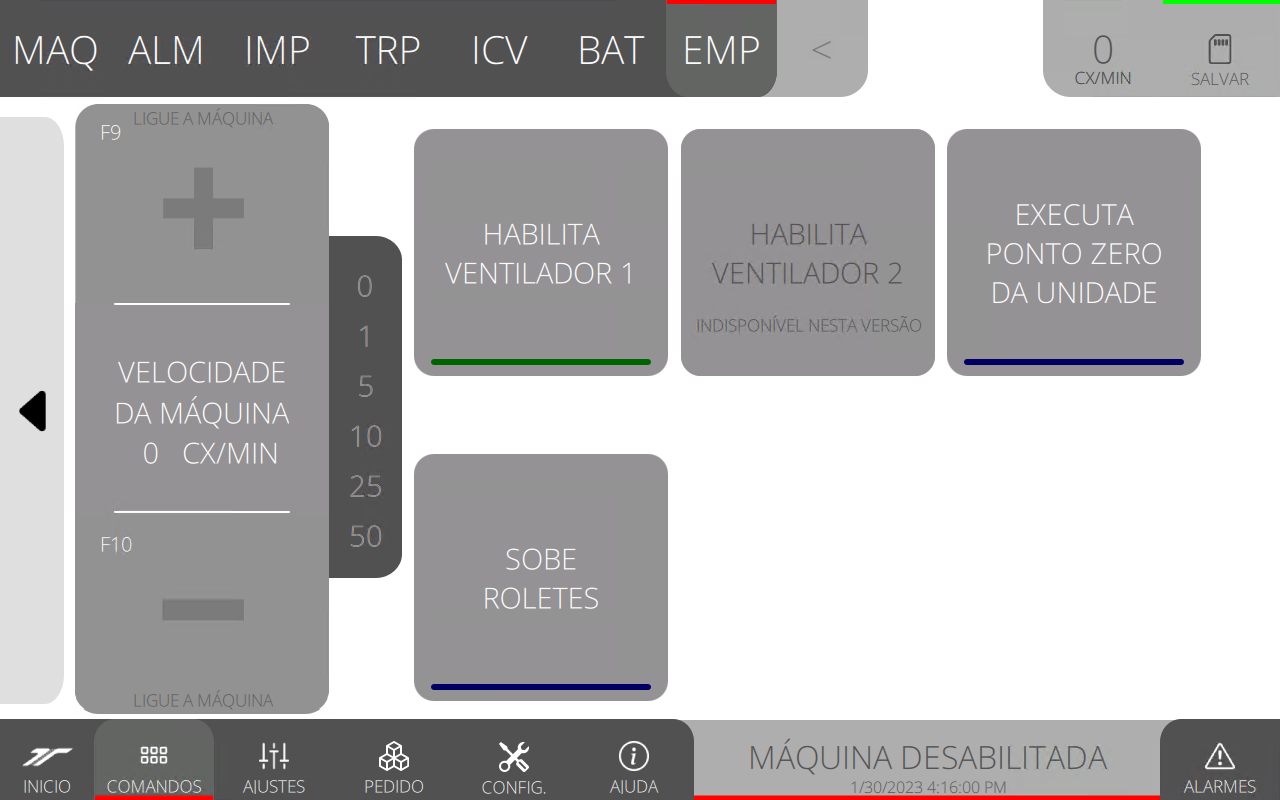
\includegraphics[width=480 px,height=300 px]{src/imagesICV/08-stacker/commands/Tela-Principal-2.png}
\end{figure}
\vspace*{\fill}


\newpage
\thispagestyle{fancy}
\vspace*{40 pt}
\subsubsection{\small{Habilita ventilador 2}} \label{sec:telaComandosEmpilhador2HabilitaVentilador2}
\vspace*{\fill}
\begin{figure}[h]
    \centering
    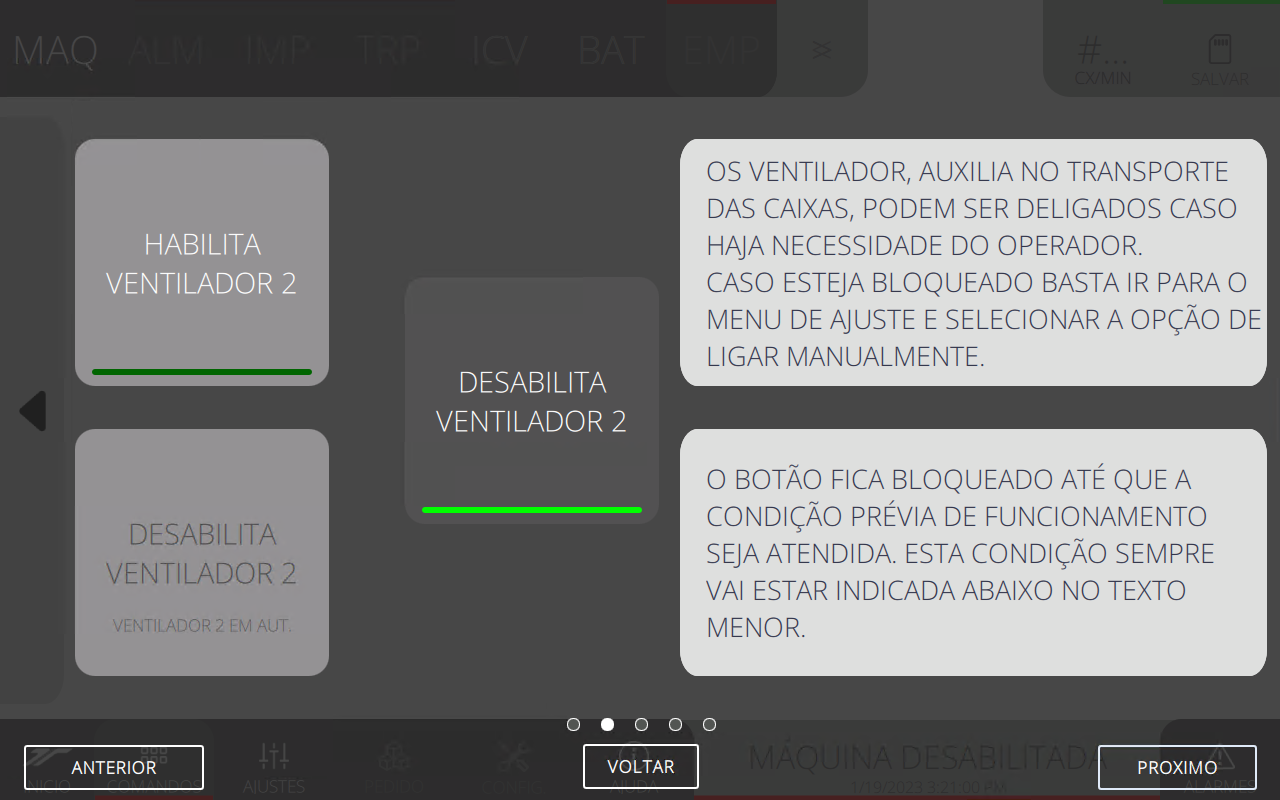
\includegraphics[width=576 px,height=360 px]{src/imagesICV/08-stacker/commands/e-2.png}
\end{figure}
\vspace*{\fill}

\newpage
\thispagestyle{fancy}
\vspace*{40 pt}
\subsubsection{\small{Desabilita ventilador 1}} \label{sec:telaComandosEmpilhador2DesabilitaVentilador1}
\vspace*{\fill}
\begin{figure}[h]
    \centering
    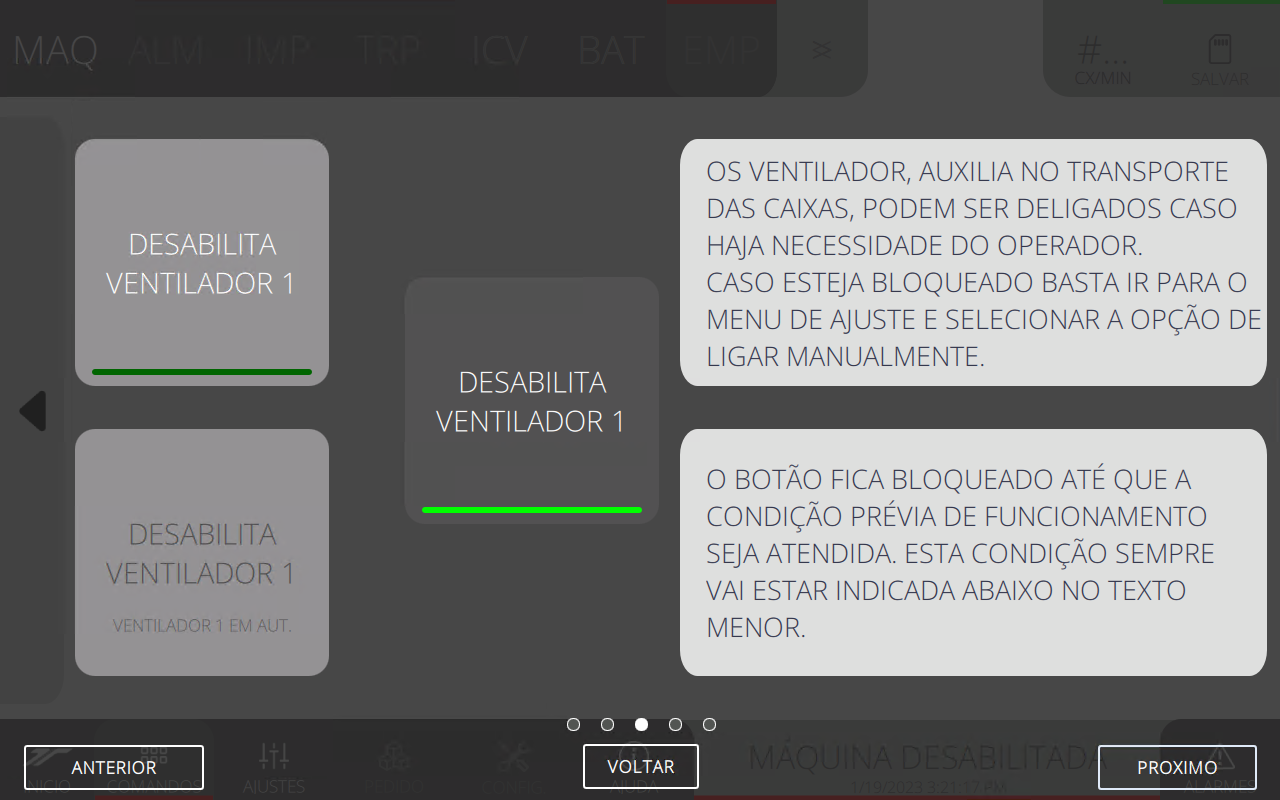
\includegraphics[width=576 px,height=360 px]{src/imagesICV/08-stacker/commands/e-3.png}
\end{figure}
\vspace*{\fill}

\newpage
\thispagestyle{fancy}
\vspace*{40 pt}
\subsubsection{\small{Executa ponto zero da unidade}} \label{sec:telaComandosEmpilhador2ExecutaPontoZeroUnidade}
\vspace*{\fill}
\begin{figure}[h]
    \centering
    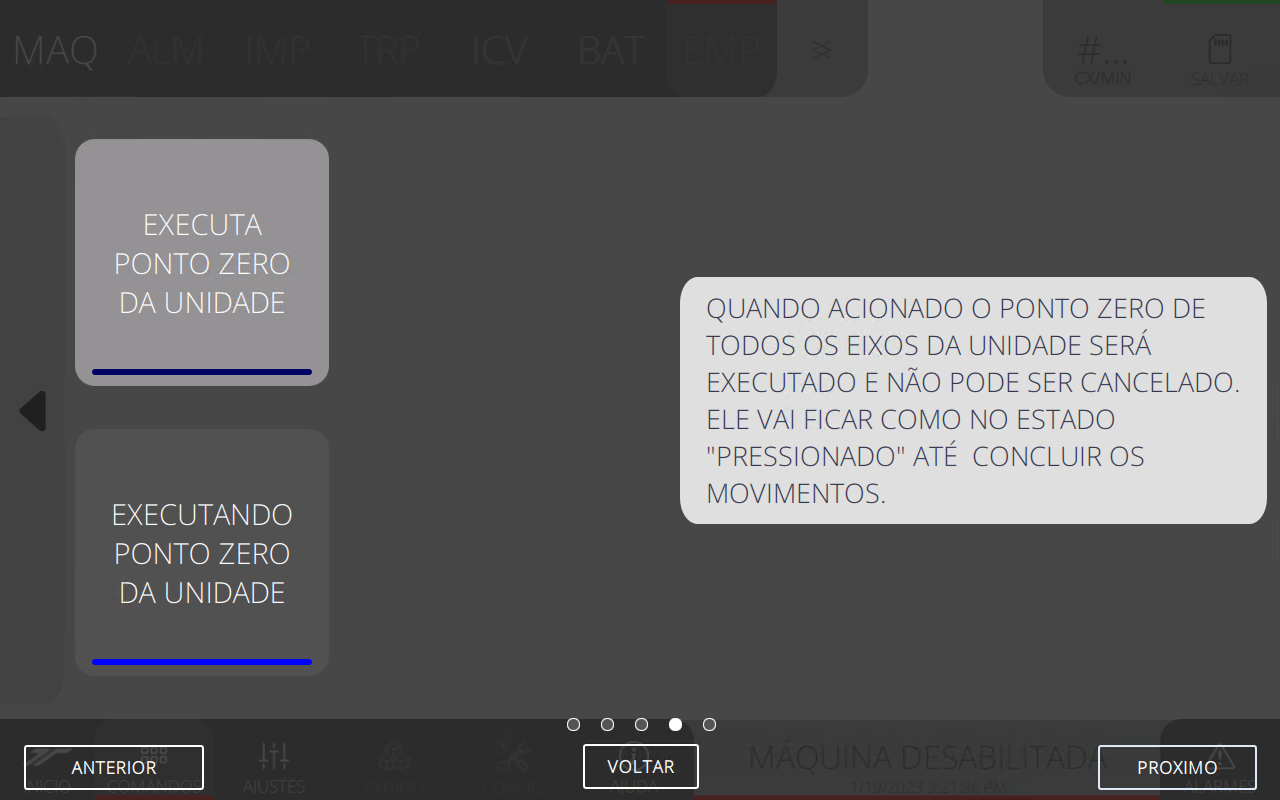
\includegraphics[width=576 px,height=360 px]{src/imagesICV/08-stacker/commands/e-4.png}
\end{figure}
\vspace*{\fill}

\newpage
\thispagestyle{fancy}
\vspace*{40 pt}
\subsubsection{\small{Habilita roletes}} \label{sec:telaComandosEmpilhador2HabilitaRoletes}
\vspace*{\fill}
\begin{figure}[h]
    \centering
    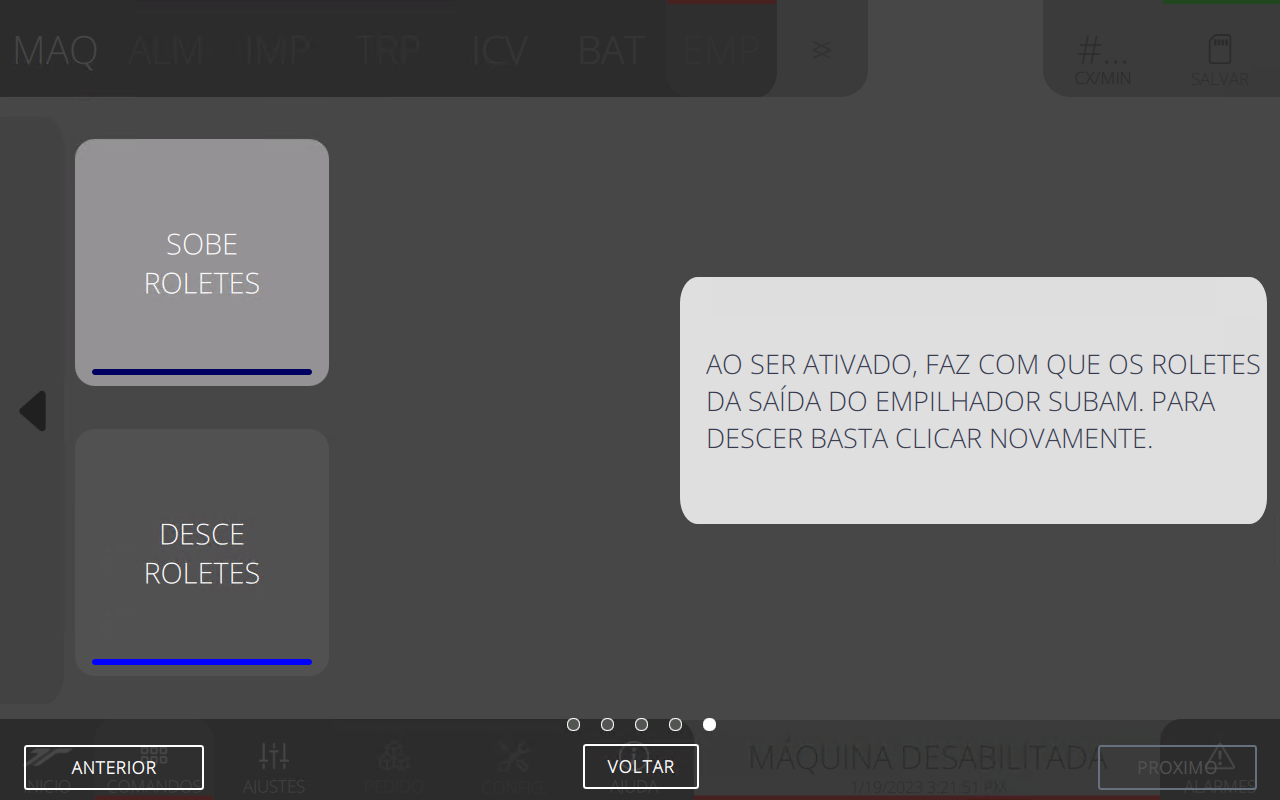
\includegraphics[width=576 px,height=360 px]{src/imagesICV/08-stacker/commands/e-5.png}
\end{figure}
\vspace*{\fill}

